% Compile either edition from its own directory with XeLaTeX.
\documentclass[11pt,a4paper]{article}
\usepackage[top=22mm,bottom=23mm,left=22mm,right=22mm,headheight=16pt,footskip=12mm]{geometry}
\usepackage{fontspec,xeCJK}
\setmainfont{TeX Gyre Pagella}
\setsansfont{TeX Gyre Heros}
\setmonofont[Scale=0.88]{Latin Modern Mono}
\IfFileExists{C:/Windows/Fonts/msyh.ttc}
  {\setCJKmainfont[AutoFakeBold=2]{SimSun}\setCJKsansfont{Microsoft YaHei}\setCJKmonofont{Microsoft YaHei}}
  {\setCJKmainfont[BoldFont=FandolSong-Bold.otf]{FandolSong-Regular.otf}%
   \setCJKsansfont[BoldFont=FandolHei-Bold.otf]{FandolHei-Regular.otf}\setCJKmonofont{FandolHei-Regular.otf}}
\usepackage{graphicx,xcolor,booktabs,tabularx,array,enumitem,fancyhdr,tikz}
\usepackage{hyperref}
\definecolor{ink}{HTML}{182F40}
\definecolor{teal}{HTML}{006D72}
\definecolor{muted}{HTML}{425B66}
\definecolor{rulecol}{HTML}{B6D0CF}
\definecolor{wash}{HTML}{EEF5F4}
\hypersetup{unicode=true,colorlinks=true,linkcolor=teal,urlcolor=teal,bookmarksnumbered=true,bookmarksdepth=2,
 pdfauthor={MULTI1Dvisual},pdftitle={MULTI1Dvisual 2.3.1 — \booktitle}}
\urlstyle{same}
\setlength{\parindent}{0pt}
\setlength{\parskip}{5.5pt}
\linespread{1.10}
\setlist[enumerate]{leftmargin=1.9em,label=\textcolor{teal}{\sffamily\bfseries\arabic*.},itemsep=3pt,topsep=4pt,parsep=0pt}
\setcounter{tocdepth}{1}
\renewcommand{\contentsname}{\tocname}
\pagestyle{fancy}\fancyhf{}
\fancyhead[L]{\small\sffamily\bfseries\color{teal}MULTI1Dvisual}
\fancyhead[R]{\small\sffamily\color{muted}\nouppercase{\leftmark}}
\fancyfoot[L]{\footnotesize\sffamily\color{muted}\booktitle\enspace ·\enspace 2.3.1}
\fancyfoot[R]{\sffamily\bfseries\color{teal}\thepage}
\renewcommand{\headrulewidth}{0.4pt}
\renewcommand{\headrule}{{\color{rulecol}\hrule height \headrulewidth width\headwidth}}
\raggedbottom
\setlength{\emergencystretch}{2em}
\newcommand{\chapterpage}[2]{\clearpage\refstepcounter{section}\label{#1}%
 \addcontentsline{toc}{section}{\protect\numberline{\thesection}#2}\markboth{#2}{}%
 {\sffamily\bfseries\color{teal}\chapterword\par}\vspace{0.5mm}
 {\sffamily\bfseries\color{ink}\fontsize{24}{30}\selectfont #2\par}\vspace{2mm}}
\newcommand{\nextpage}[2]{\clearpage\phantomsection\label{#1}%
 \pdfbookmark[2]{#2}{sub:#1}%
 {\sffamily\bfseries\color{teal}\chapterword\par}\vspace{0.5mm}
 {\sffamily\bfseries\color{ink}\fontsize{22}{28}\selectfont #2\par}\vspace{2mm}}
\newcommand{\subhead}[1]{\par\addvspace{2.5mm}{\large\sffamily\bfseries\color{teal}#1\par}\nobreak}
\newcommand{\ui}[1]{{\sffamily\bfseries\color{ink}#1}}
\newcommand{\code}[1]{{\ttfamily\detokenize{#1}}}
\newcommand{\keys}[1]{{\small\sffamily\bfseries #1}}
\newcommand{\checknote}[2]{\par\addvspace{2.5mm}\noindent\colorbox{wash}{%
 \parbox{\dimexpr\linewidth-2\fboxsep\relax}{\vspace{1mm}\hspace{1.4mm}%
 \begin{minipage}{\dimexpr\linewidth-3mm\relax}{\sffamily\bfseries\color{teal}#1}\enspace #2\end{minipage}\vspace{1.4mm}}}\par}
\newcommand{\Table}[3]{\par\smallskip\begingroup\small\renewcommand{\arraystretch}{1.24}%
 \begin{tabularx}{\linewidth}{@{}>{\raggedright\arraybackslash}p{.295\linewidth}>{\raggedright\arraybackslash}X@{}}\toprule
 \sffamily\bfseries\color{teal}#1 & \sffamily\bfseries\color{teal}#2\\\midrule #3\bottomrule
 \end{tabularx}\endgroup\par}
\newcounter{manualfig}
\newcommand{\Figure}[3]{\par\addvspace{2mm}\stepcounter{manualfig}\begingroup\centering
 \includegraphics[width=\linewidth,height=#3,keepaspectratio]{images/#1.png}\par
 \endgroup{\small\color{muted}{\sffamily\bfseries\color{teal}\figword\ \themanualfig.}\enspace #2\par}\smallskip}
\newcommand{\repo}{\href{https://github.com/boxu-pku/MULTI1Dvisual}{GitHub · boxu-pku/MULTI1Dvisual}}
\newcommand{\cover}{\thispagestyle{empty}\vspace*{6mm}
 
\includegraphics[width=27mm]{../../resources/icons/multi1dvisual.png}\par\vspace{9mm}
 {\sffamily\bfseries\color{ink}\fontsize{38}{44}\selectfont MULTI1Dvisual\par}
 {\sffamily\bfseries\color{teal}\fontsize{28}{37}\selectfont\booktitle\par}
 \vspace{3mm}{\Large\color{muted}\coverline\par}
 \vfill
 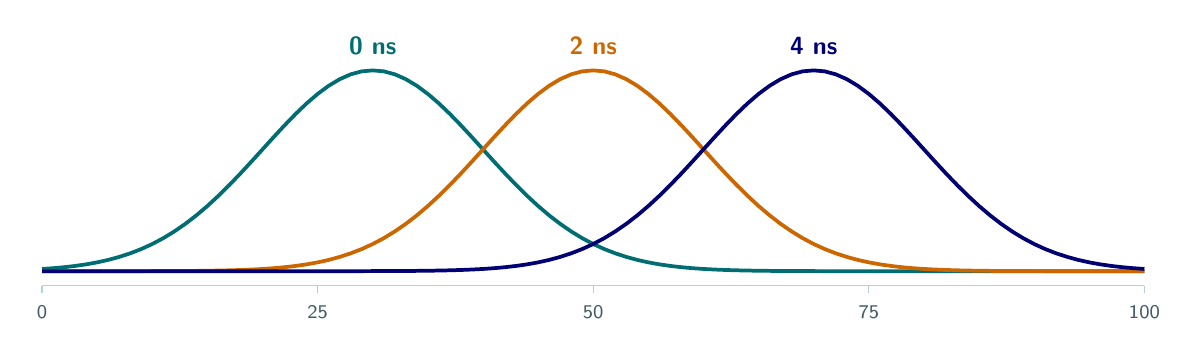
\begin{tikzpicture}[x=.140cm,y=.51cm]
 \draw[rulecol] (0,0)--(100,0);
 \foreach \p in {0,25,50,75,100} {
  \draw[rulecol] (\p,0)--(\p,-.18);
  \node[below,font=\scriptsize\sffamily,text=muted] at (\p,-.25){\p};}
 \foreach \p/\col/\name in {30/teal/0,50/orange!80!black/2,70/blue!45!black/4}{
  \draw[line width=1.35pt,color=\col] plot[domain=0:100,samples=101] (\x,{.36+5*exp(-((\x-\p)^2)/200)});
  \node[above,font=\small\sffamily\bfseries,text=\col] at (\p,5.52){\name\ ns};}
 \end{tikzpicture}\par
 {\small\color{muted}\covercaption\par}
 \vfill{\color{rulecol}\rule{\linewidth}{0.8pt}}\par
 {\large\sffamily\bfseries\color{ink}\editionline}\hfill{\sffamily\color{muted}\manualdate}\par
 {\small\color{muted}\creditline}\clearpage}
\newcommand{\contentspage}{\markboth{\tocname}{}\pdfbookmark[1]{\tocname}{contents}%
 \tableofcontents}
